
\documentclass[11pt,a4paper,UTF8]{ctexart}
\usepackage[T1]{fontenc}
\usepackage[utf8]{inputenc}
\usepackage{authblk}

\title{Expert C++}
\author{Vardan Grigoryan \& Shunguang Wu}
\date{\today}

\usepackage{ctex} %导入中文包
\usepackage{tocvsec2}

\usepackage{graphicx}
\usepackage{subfigure}

\usepackage{subfiles} %使用多文件方式进行

\usepackage{geometry} %设置页边距的包
\geometry{left=2.5cm,right=2cm,top=2.54cm,bottom=2.54cm} %设置书籍的页边距

\usepackage{hyperref}  %制作pdf的目录
\hypersetup{hidelinks, %去红框
	colorlinks=true,
	allcolors=black,
	pdfstartview=Fit,
	breaklinks=true
}

% 调整itemlist中的行间距
\usepackage{enumitem}
\setenumerate[1]{itemsep=0pt,partopsep=0pt,parsep=\parskip,topsep=5pt}
\setitemize[1]{itemsep=0pt,partopsep=0pt,parsep=\parskip,topsep=5pt}
\setdescription{itemsep=0pt,partopsep=0pt,parsep=\parskip,topsep=5pt}

% 超链接样式设置
\usepackage{hyperref}
\hypersetup{
	colorlinks=true,
	linkcolor=blue,
	filecolor=blue,
	urlcolor=blue,
	citecolor=cyan,
}

\usepackage{indentfirst}

\begin{document}
	%\maketitle
	
	\begin{center}
		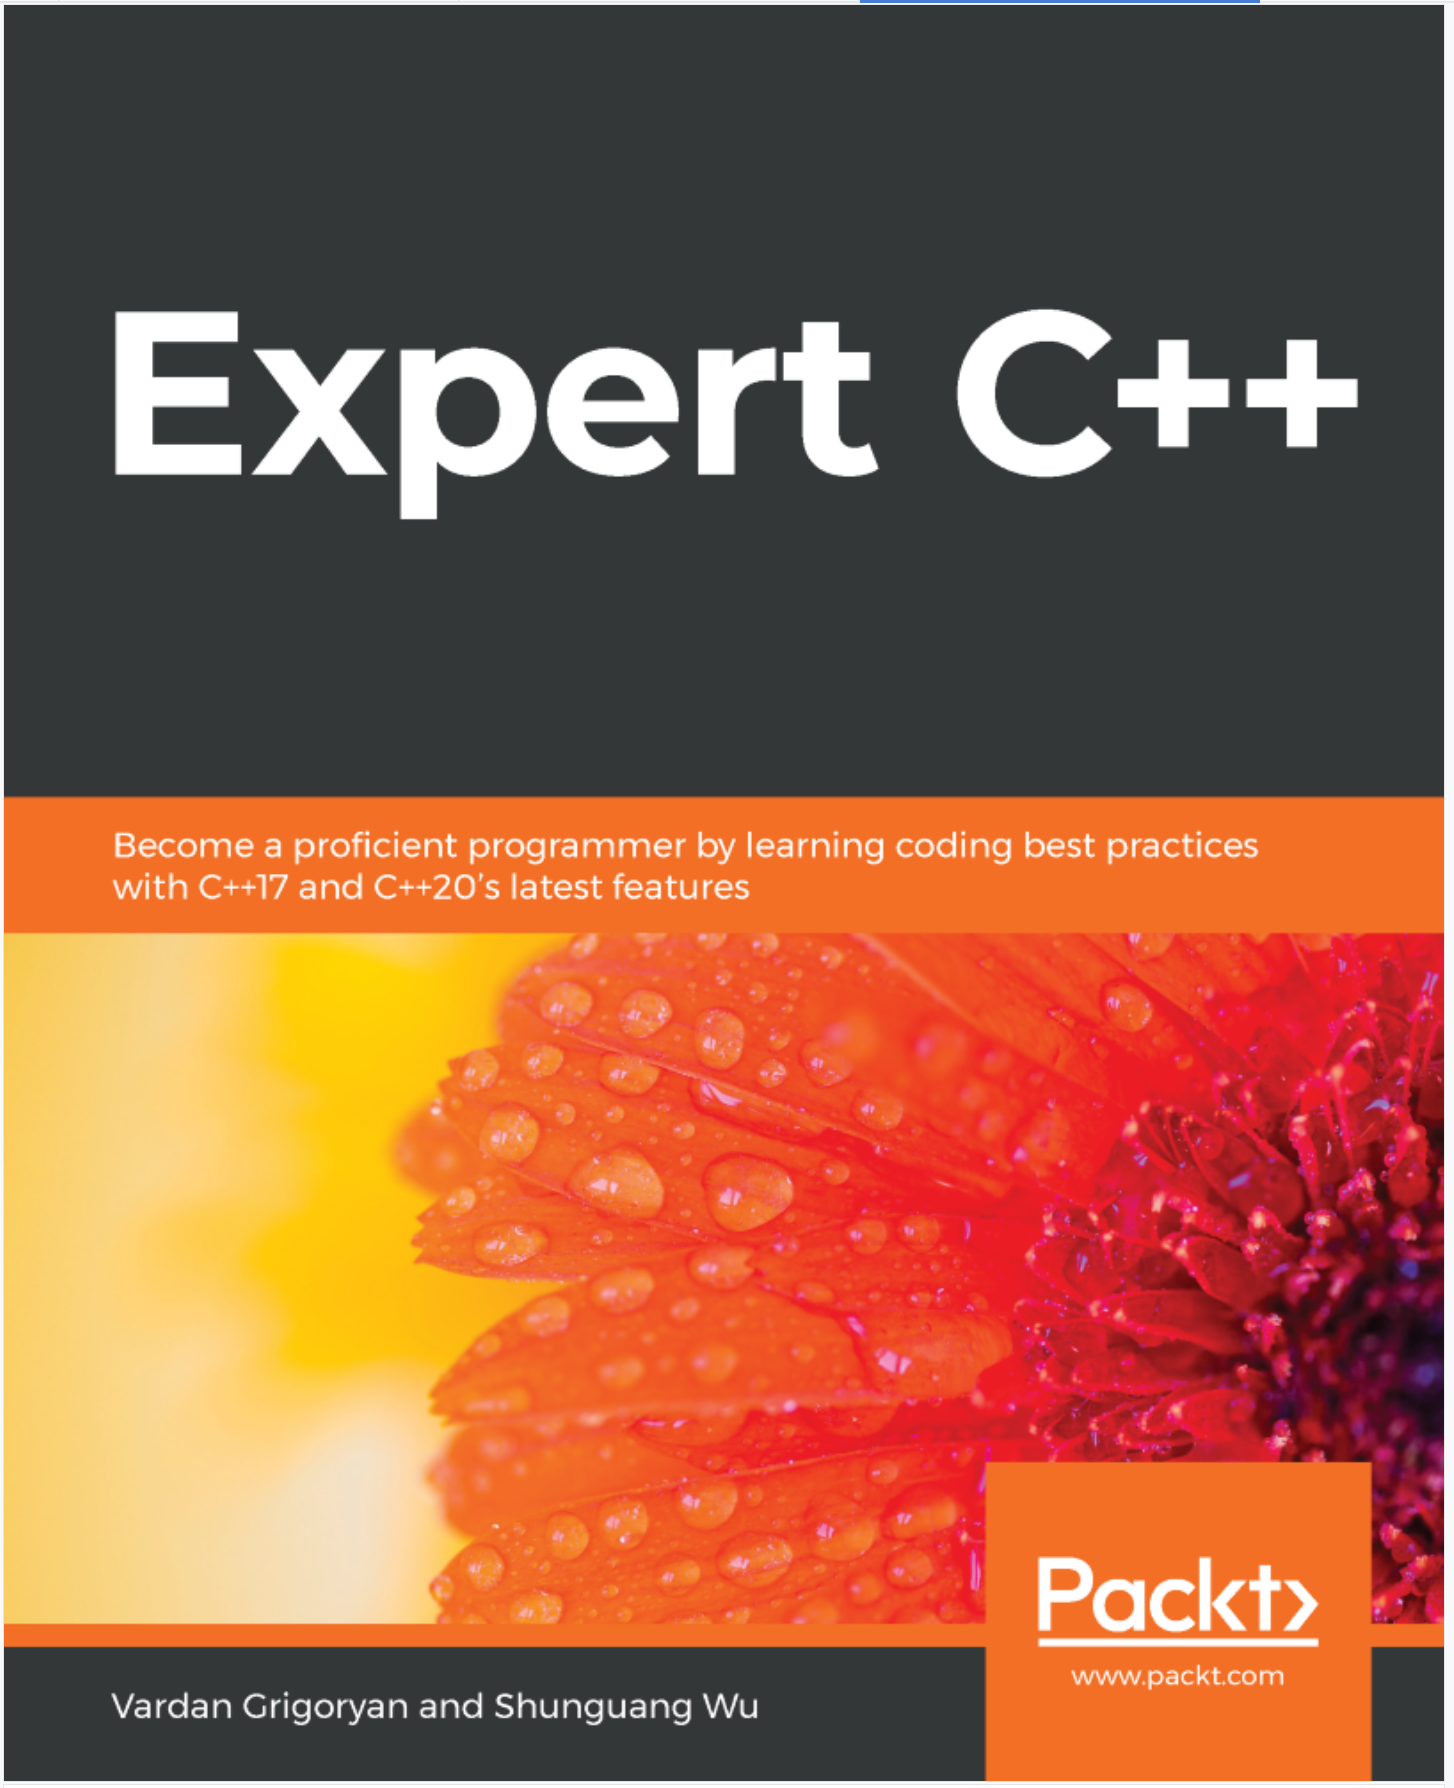
\includegraphics[width=1\textwidth]{images/cover}
		\newpage
		\huge
		\textbf{Expert C++} 
		\\[9pt]
		\normalsize
		Become a proficient programmer by learning coding best practices with C++17 and C++20's latest features
		\\[10pt]
		\normalsize 
		作者: Vardan Grigoryan 和 Shunguang Wu
		\\[8pt]
		\normalsize
		译者;陈晓伟
	\end{center}

	
	\hspace*{\fill} \\ %插入空行
	\noindent\textbf{本书主旨}\ 
	\begin{itemize}
		\item 通过学习函数式编程、模板和网络等高级概念,设计专业的、可维护的应用。
		\item 应用设计模式和最佳实践来解决实际问题。
		\item 通过设计并发数据结构和算法提升应用性能。
	\end{itemize}
	
	\hspace*{\fill} \\ %插入空行
	\noindent\textbf{本书概述}\ \par
	C++经过多年的发展,目前的最新标准为C++20。自C++11以来,C++语言不断的增强特性集。在新标准中,您将了解到一系列新特性,如概念、模块、范围和协程。这本书将作为学习错综复杂的语言、技术、C++工具和C++ 20新特性的指南,同时也会帮助你了解,在构建软件时如何应用他们。\par
	
	本书将从C++的最新特性开始,然后转向高级技术,如多线程、并发性、调试、监视和高性能编程。本书将深入探讨面向对象的编程原理和C++标准模板库,并展示如何创建自定义模板。之后,将学习不同的方法,比如测试驱动开发(TDD)、行为驱动开发(BDD)和领域驱动设计(DDD),然后看看构建专业级应用程序所必需的编码最佳实践和设计模式。本书的最后,有关于人工智能和机器学习的C++最新进展的内容。\par
	
	这本书的末尾,还有实际应用程序开发方面的专业知识,包括设计复杂软件的过程。\par
	
	\hspace*{\fill} \\ %插入空行
	\noindent\textbf{将会学到}\ \par
	\begin{itemize}
		\item 了解内存管理和C++底层编程,编写安全稳定的应用程序。
		\item 了解C++20的新特性,如模块、概念、范围和协程。
		\item 熟悉调试和测试技术,减少程序中的问题。
		\item 使用Qt5设计带GUI的程序。
		\item 使用多线程和并发性可以使程序运行得更快。
		\item 使用C++的面向对象的功能开发高端游戏。
		\item 使用C++探索人工智能和机器学习。
	\end{itemize}

	\hspace*{\fill} \\ %插入空行
	\noindent\textbf{目标读者}\ \par
	这本书是为有经验的C++开发人员准备的,能将他们现有的知识进行升级,并完善在构建专业级应用程序方面的技能。\par
	
	\hspace*{\fill} \\ %插入空行
	\noindent\textbf{作者简介}\ \par
	\textbf{Vardan Grigoryan}是一名高级后端工程师和C++开发者,拥有9年以上的开发经验。Vardan以C++开发人员的身份开始他的职业生涯,然后转到服务器端后端开发领域。在设计可伸缩的后端架构时,总是在耗时敏感的关键部分使用C++。Vardan喜欢在更深的层面上处理计算机系统和程序结构,通过对现有解决方案的详细分析和对复杂系统的精心设计,可以实现真正的卓越编程。\par
	
	\textbf{Shunguang Wu}是美国约翰霍普金斯大学应用物理实验室高级专业人员,分别在西北大学和美国莱特州立大学获得理论物理和电气工程博士学位。早期职业生涯中,在非线性动力学、统计信号处理和计算机视觉领域发表了大约50篇评论期刊论文。与C++的邂逅是在20世纪90年代末的本科教学中,从那时起,他就一直在学术和工业实验室使用C++设计和开发大量的研究和开发。这些项目都是跨平台项目,主要是Windows和Linux平台。\par
	
	\hspace*{\fill} \\ %插入空行
	\noindent\textbf{书评人简介}\ \par
	\textbf{Lou Mauget}在密歇根州立大学(Michigan State University)主修物理时,使用软件设计了回旋加速器。之后,在IBM工作了34年,目前是堪萨斯州利伍德的Keyhole软件公司的顾问。Lou会使用C++、Java、JavaScript、Python和新语言进行了编程,几乎是个语言通。其目前的关注的领域有,响应式函数编程、容器、Node.js, NoSQL,地理空间系统,移动端,以及任何新的语言或框架。与其他人合著了三本计算机相关的书籍。他编写了两个IBM DeveloperWorks XML教程,并与其他人合作为IBM编写了几个J2EE认证测试。并且,他还是Packt Publishing等公司的书评人。 \par
	
	\textbf{Scott Hutchinson}在加州奥克斯纳德领导着一个C++和F\#开发团队。做了几年VB/VBA开发人员之后,他在2002年开始使用.NET框架。2016年之后,他的大部分开发工作都用C++完成。他是\href{https://github.com/exercism/fsharp}{F\# track on Exercism}项目的导师,并在工作中作为团队教授F\#函数式编程。他的主要关注函数式编程和机器学习。并且,他在假期时,会常在南加州的山区进行徒步旅行。 \par
	
	\hspace*{\fill} \\ %插入空行
	\noindent\textbf{本书相关}\ \par
	\begin{itemize}
		\item github翻译地址:\href{https://github.com/xiaoweiChen/Expert-Cpp}{https://github.com/xiaoweiChen/Expert-Cpp}
		\item 英文原版PDF:\href{https://zh.1lib.us/book/5537006/2e05c8}{https://zh.1lib.us/book/5537006/2e05c8}
	\end{itemize}
	\newpage
	
	\tableofcontents
	\newpage
	
	\setsecnumdepth{section}
	\section{C++编程基础}
		\subfile{content/Section-1/summary.tex}
		\subsection{第1章:构建C++应用}
			\subfile{content/Section-1/Chapter-1/chapter1.tex}
		\subsection{第2章:C++底层编程}
			\subfile{content/Section-1/Chapter-2/chapter2.tex}
		\subsection{第3章:面向对象编程}
			\subfile{content/Section-1/Chapter-3/chapter3.tex}
		\subsection{第4章:了解并设计模板}
			\subfile{content/Section-1/Chapter-4/chapter4.tex}
		\subsection{第5章:内存管理和智能指针}
			\subfile{content/Section-1/Chapter-5/chapter5.tex}
	\section{设计健壮和高效的应用}
		\subfile{content/Section-2/summary.tex}
		\subsection{第6章:构建C++应用}
			\subfile{content/Section-2/Chapter-6/chapter6.tex}
		\subsection{第7章:C++底层编程}
			\subfile{content/Section-2/Chapter-7/chapter7.tex}
		\subsection{第8章:面向对象编程}
			\subfile{content/Section-2/Chapter-8/chapter8.tex}
		\subsection{第9章:了解并设计模板}
			\subfile{content/Section-2/Chapter-9/chapter9.tex}
		\subsection{第10章:内存管理和智能指针}
			\subfile{content/Section-2/Chapter-10/chapter10.tex}
		\subsection{第11章:构建C++应用}
			\subfile{content/Section-2/Chapter-11/chapter11.tex}
		\subsection{第12章:C++底层编程}
			\subfile{content/Section-2/Chapter-12/chapter12.tex}
		\subsection{第13章:面向对象编程}
			\subfile{content/Section-2/Chapter-13/chapter13.tex}
		\subsection{第14章:了解并设计模板}
			\subfile{content/Section-2/Chapter-14/chapter14.tex}
	\section{人工智能领域中的C++}
		\subfile{content/Section-3/summary.tex}
		\subsection{第15章:使用C++进行机器学习}
			\subfile{content/Section-3/Chapter-15/chapter15.tex}
		\subsection{第16章:实现一个交互式搜索引擎}
			\subfile{content/Section-3/Chapter-16/chapter16.tex}

\end{document}